% Options for packages loaded elsewhere
\PassOptionsToPackage{unicode}{hyperref}
\PassOptionsToPackage{hyphens}{url}
%
\documentclass[
]{article}
\usepackage{amsmath,amssymb}
\usepackage{lmodern}
\usepackage{iftex}
\ifPDFTeX
  \usepackage[T1]{fontenc}
  \usepackage[utf8]{inputenc}
  \usepackage{textcomp} % provide euro and other symbols
\else % if luatex or xetex
  \usepackage{unicode-math}
  \defaultfontfeatures{Scale=MatchLowercase}
  \defaultfontfeatures[\rmfamily]{Ligatures=TeX,Scale=1}
\fi
% Use upquote if available, for straight quotes in verbatim environments
\IfFileExists{upquote.sty}{\usepackage{upquote}}{}
\IfFileExists{microtype.sty}{% use microtype if available
  \usepackage[]{microtype}
  \UseMicrotypeSet[protrusion]{basicmath} % disable protrusion for tt fonts
}{}
\makeatletter
\@ifundefined{KOMAClassName}{% if non-KOMA class
  \IfFileExists{parskip.sty}{%
    \usepackage{parskip}
  }{% else
    \setlength{\parindent}{0pt}
    \setlength{\parskip}{6pt plus 2pt minus 1pt}}
}{% if KOMA class
  \KOMAoptions{parskip=half}}
\makeatother
\usepackage{xcolor}
\usepackage[margin=1in]{geometry}
\usepackage{color}
\usepackage{fancyvrb}
\newcommand{\VerbBar}{|}
\newcommand{\VERB}{\Verb[commandchars=\\\{\}]}
\DefineVerbatimEnvironment{Highlighting}{Verbatim}{commandchars=\\\{\}}
% Add ',fontsize=\small' for more characters per line
\usepackage{framed}
\definecolor{shadecolor}{RGB}{248,248,248}
\newenvironment{Shaded}{\begin{snugshade}}{\end{snugshade}}
\newcommand{\AlertTok}[1]{\textcolor[rgb]{0.94,0.16,0.16}{#1}}
\newcommand{\AnnotationTok}[1]{\textcolor[rgb]{0.56,0.35,0.01}{\textbf{\textit{#1}}}}
\newcommand{\AttributeTok}[1]{\textcolor[rgb]{0.77,0.63,0.00}{#1}}
\newcommand{\BaseNTok}[1]{\textcolor[rgb]{0.00,0.00,0.81}{#1}}
\newcommand{\BuiltInTok}[1]{#1}
\newcommand{\CharTok}[1]{\textcolor[rgb]{0.31,0.60,0.02}{#1}}
\newcommand{\CommentTok}[1]{\textcolor[rgb]{0.56,0.35,0.01}{\textit{#1}}}
\newcommand{\CommentVarTok}[1]{\textcolor[rgb]{0.56,0.35,0.01}{\textbf{\textit{#1}}}}
\newcommand{\ConstantTok}[1]{\textcolor[rgb]{0.00,0.00,0.00}{#1}}
\newcommand{\ControlFlowTok}[1]{\textcolor[rgb]{0.13,0.29,0.53}{\textbf{#1}}}
\newcommand{\DataTypeTok}[1]{\textcolor[rgb]{0.13,0.29,0.53}{#1}}
\newcommand{\DecValTok}[1]{\textcolor[rgb]{0.00,0.00,0.81}{#1}}
\newcommand{\DocumentationTok}[1]{\textcolor[rgb]{0.56,0.35,0.01}{\textbf{\textit{#1}}}}
\newcommand{\ErrorTok}[1]{\textcolor[rgb]{0.64,0.00,0.00}{\textbf{#1}}}
\newcommand{\ExtensionTok}[1]{#1}
\newcommand{\FloatTok}[1]{\textcolor[rgb]{0.00,0.00,0.81}{#1}}
\newcommand{\FunctionTok}[1]{\textcolor[rgb]{0.00,0.00,0.00}{#1}}
\newcommand{\ImportTok}[1]{#1}
\newcommand{\InformationTok}[1]{\textcolor[rgb]{0.56,0.35,0.01}{\textbf{\textit{#1}}}}
\newcommand{\KeywordTok}[1]{\textcolor[rgb]{0.13,0.29,0.53}{\textbf{#1}}}
\newcommand{\NormalTok}[1]{#1}
\newcommand{\OperatorTok}[1]{\textcolor[rgb]{0.81,0.36,0.00}{\textbf{#1}}}
\newcommand{\OtherTok}[1]{\textcolor[rgb]{0.56,0.35,0.01}{#1}}
\newcommand{\PreprocessorTok}[1]{\textcolor[rgb]{0.56,0.35,0.01}{\textit{#1}}}
\newcommand{\RegionMarkerTok}[1]{#1}
\newcommand{\SpecialCharTok}[1]{\textcolor[rgb]{0.00,0.00,0.00}{#1}}
\newcommand{\SpecialStringTok}[1]{\textcolor[rgb]{0.31,0.60,0.02}{#1}}
\newcommand{\StringTok}[1]{\textcolor[rgb]{0.31,0.60,0.02}{#1}}
\newcommand{\VariableTok}[1]{\textcolor[rgb]{0.00,0.00,0.00}{#1}}
\newcommand{\VerbatimStringTok}[1]{\textcolor[rgb]{0.31,0.60,0.02}{#1}}
\newcommand{\WarningTok}[1]{\textcolor[rgb]{0.56,0.35,0.01}{\textbf{\textit{#1}}}}
\usepackage{graphicx}
\makeatletter
\def\maxwidth{\ifdim\Gin@nat@width>\linewidth\linewidth\else\Gin@nat@width\fi}
\def\maxheight{\ifdim\Gin@nat@height>\textheight\textheight\else\Gin@nat@height\fi}
\makeatother
% Scale images if necessary, so that they will not overflow the page
% margins by default, and it is still possible to overwrite the defaults
% using explicit options in \includegraphics[width, height, ...]{}
\setkeys{Gin}{width=\maxwidth,height=\maxheight,keepaspectratio}
% Set default figure placement to htbp
\makeatletter
\def\fps@figure{htbp}
\makeatother
\setlength{\emergencystretch}{3em} % prevent overfull lines
\providecommand{\tightlist}{%
  \setlength{\itemsep}{0pt}\setlength{\parskip}{0pt}}
\setcounter{secnumdepth}{-\maxdimen} % remove section numbering
\ifLuaTeX
  \usepackage{selnolig}  % disable illegal ligatures
\fi
\IfFileExists{bookmark.sty}{\usepackage{bookmark}}{\usepackage{hyperref}}
\IfFileExists{xurl.sty}{\usepackage{xurl}}{} % add URL line breaks if available
\urlstyle{same} % disable monospaced font for URLs
\hypersetup{
  pdftitle={Taller Evaluable 1, FIFA 2022-23},
  hidelinks,
  pdfcreator={LaTeX via pandoc}}

\title{Taller Evaluable 1, FIFA 2022-23}
\author{}
\date{\vspace{-2.5em}}

\begin{document}
\maketitle

\begin{center}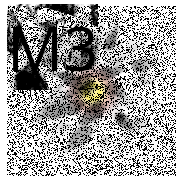
\includegraphics[width=0.1\linewidth]{logoM3} \end{center}

\hypertarget{taller-evaluable-datos-fifa-2023}{%
\section{Taller evaluable datos FIFA
2023}\label{taller-evaluable-datos-fifa-2023}}

Cada pregunta vale 1 punto menos las dos últimas que valen 1.5 puntos.
Se puntúa la presentación, la claridad y que los dibujos están
completos. Este taller está pensado para resolver con R-base pero podéis
utilizar tidyverse u otros paquetes de R.

En la web de kaggle
\href{https://www.kaggle.com/datasets/bryanb/fifa-player-stats-database}{FIFA23
OFFICIAL DATASET}. Contiene todos los data sets de de datos básicos de
FIFA17 to FIFA23 del videojuego.

Las siguientes preguntas son relativas al data set
\texttt{players\_23.csv}, que se adjunta con la práctica.

Hay que contestar con código R explicar adecuadamente cada salida. Subid
a la activad el Rmd y el html.

Rellenad estos datos:

\textbf{PONED NOMBRE DEL GRUPO}

\begin{itemize}
\tightlist
\item
  Florit Ensenyat, Jordi
\item
  Ferrer Fernández, Marc
\item
  Girón Rodríguez, Pau
\item
  Fornés Reynés, Josep Gabriel
\end{itemize}

\hypertarget{carga-de-datos}{%
\subsection{Carga de datos}\label{carga-de-datos}}

Tenéis que carga los datos con el código que se ve a continuación.
Visualizar y explorara el data set y averiguar de qué tipo son cada una
de las variables y en qué tipo de fichero están guardadas. El código
carga los datos en un data frame llamado \texttt{datos} con la función
\texttt{read.csv}. Debéis entender clases y tipos de datos de cada de
cada columna de datos. El parámetro \texttt{encoding} es necesario para
cargar debidamente los acentos y caracteres especiales. Lo que obtenemos
es un data frame de 18539 observaciones (filas) y 90 variables
(columnas).

Cargaremos todas las variables de texto como factor con el parámetro
\texttt{stringsAsFactors\ =\ TRUE}

\begin{Shaded}
\begin{Highlighting}[]
\NormalTok{datos }\OtherTok{=} \FunctionTok{read.csv}\NormalTok{(}\StringTok{"players\_fifa23.csv"}\NormalTok{,}
  \AttributeTok{encoding=}\StringTok{"UTF{-}8"}\NormalTok{,}\AttributeTok{stringsAsFactors =} \ConstantTok{TRUE}\NormalTok{)}\CommentTok{\# cambia tu path}
\CommentTok{\#str(datos)}
\CommentTok{\#names(datos)}
\end{Highlighting}
\end{Shaded}

Las variables de la 1 (\texttt{NationalTeam}) a la
31(\texttt{NationalPosition}) son variables de perfil del jugador: su
nombre, su equipo su sueldo su número de camiseta\ldots{} El resto de
variables de la 34 (\texttt{pace}) a la 90 (\texttt{rb}) son variables
numéricas enteras con valores de 0 a 100 que parametrizan cómo es el
jugador el el juego FIFA player 2023.

\hypertarget{pregunta-1}{%
\subsection{Pregunta 1}\label{pregunta-1}}

Las selecciones europeas que han ganado un mundial son

\begin{Shaded}
\begin{Highlighting}[]
\NormalTok{eur}\OtherTok{=}\FunctionTok{c}\NormalTok{(}\StringTok{"England"}\NormalTok{,}\StringTok{"France"}\NormalTok{,}\StringTok{"Germany"}\NormalTok{,}\StringTok{"Italy"}\NormalTok{,}\StringTok{"Portugal"}\NormalTok{,}\StringTok{"Spain"}\NormalTok{)}
\NormalTok{eur}
\end{Highlighting}
\end{Shaded}

\begin{verbatim}
## [1] "England"  "France"   "Germany"  "Italy"    "Portugal" "Spain"
\end{verbatim}

Generar un data frame con el nombre \texttt{fifa23\_eur} con los
jugadores de estas selecciones.

\hypertarget{soluciuxf3n-1}{%
\subsubsection{Solución 1}\label{soluciuxf3n-1}}

\begin{Shaded}
\begin{Highlighting}[]
\NormalTok{fifa23\_eur }\OtherTok{=}\NormalTok{ datos[datos}\SpecialCharTok{$}\NormalTok{NationalTeam }\SpecialCharTok{\%in\%}\NormalTok{ eur,]}
\NormalTok{fifa23\_eur}\SpecialCharTok{$}\NormalTok{NationalTeam }\OtherTok{=} \FunctionTok{droplevels}\NormalTok{(fifa23\_eur}\SpecialCharTok{$}\NormalTok{NationalTeam)}
\FunctionTok{unique}\NormalTok{(fifa23\_eur}\SpecialCharTok{$}\NormalTok{Name)}
\end{Highlighting}
\end{Shaded}

\begin{verbatim}
##   [1] K. Benzema        K. Mbappé         M. Neuer          Cristiano Ronaldo
##   [5] H. Kane           J. Kimmich        N. Kanté          Rúben Dias       
##   [9] G. Donnarumma     Bernardo Silva    João Cancelo      M. ter Stegen    
##  [13] A. Rüdiger        Rodri             H. Lloris         T. Müller        
##  [17] De Gea            M. Verratti       M. Maignan        L. Goretzka      
##  [21] C. Immobile       R. Sterling       K. Trapp          Bruno Fernandes  
##  [25] A. Laporte        K. Coman          N. Barella        C. Nkunku        
##  [29] N. Süle           S. Gnabry         İ. Gündoğan       K. Walker        
##  [33] Jordi Alba        Sergio Busquets   P. Pogba          Jorginho         
##  [37] Gerard Moreno     Pedri             P. Foden          T. Hernández     
##  [41] Diogo Jota        M. Reus           L. Hernández      Sergio Ramos     
##  [45] D. Berardi        J. Grealish       Carvajal          R. Varane        
##  [49] W. Ben Yedder     L. Insigne        K. Trippier       L. Bonucci       
##  [53] J. Bellingham     F. Chiesa         Rafael Leão       J. Koundé        
##  [57] L. Sané           R. James          A. Bastoni        K. Havertz       
##  [61] João Félix        D. Rice           M. Mount          J. Sancho        
##  [65] Oyarzabal         L. Pellegrini     Marcos Llorente   Rúben Neves      
##  [69] P. Kimpembe       Unai Simón        Carlos Soler      Pau Torres       
##  [73] J. Henderson      A. Griezmann      J. Stones         Koke             
##  [77] G. Di Lorenzo     M. Locatelli      R. Gosens         Gonçalo Guedes   
##  [81] J. Brandt         T. Werner         Gayà              Otávio           
##  [85] R. Guerreiro      T. Abraham        N. Schlotterbeck  B. Saka          
##  [89] Dani Olmo         A. Tchouaméni     Ferran Torres     A. Ramsdale      
##  [93] B. Chilwell       André Silva       J. Pickford       Rui Patrício     
##  [97] Azpilicueta       L. Digne          L. Spinazzola     A. Lopes         
## [101] F. Acerbi         D. Raum           A. Areola         J. Musiala       
## [105] Pablo Sarabia     H. Maguire        Palhinha          N. Pope          
## [109] João Moutinho     Pepe              J. Hofmann        K. Phillips      
## [113] M. Guendouzi      Nuno Mendes       W. Saliba         J. Clauss        
## [117] Danilo Pereira    Morata            José Fonte        L. Klostermann   
## [121] B. Cristante      A. Belotti        A. Rabiot         C. Gallagher     
## [125] Matheus Nunes     G. Raspadori      B. Pavard         Diogo Costa      
## [129] C. Coady          A. Florenzi       M. Kean           A. Meret         
## [133] L. Nmecha         S. Sirigu         Eric García       Robert Sánchez   
## [137] Emerson           T. Kehrer        
## 17530 Levels: A. Abaz A. Abdallah A. Abdennour A. Abdi A. Abdijanovic ... Zubimendi
\end{verbatim}

\hypertarget{pregunta-2}{%
\subsection{Pregunta 2}\label{pregunta-2}}

Calcular la media y la desviación típica del valor de cada selección
nacional cada equipo del data frame \texttt{fifa23\_eur}.

Calcular la media y la desviación típica EN MILES de euros del valor de
cada jugador \texttt{ValueEUR} de cada selección nacional del frame
\texttt{fifa23\_eur} por posición en el campo delantera media y defensa.

\hypertarget{solucion-2}{%
\subsubsection{Solucion 2}\label{solucion-2}}

\hypertarget{pregunta-3}{%
\subsection{Pregunta 3}\label{pregunta-3}}

Discretiza la variable \texttt{ValueEUR} de \texttt{fifa23\_eur} en los
4 niveles siguientes: ``Cuartil\_1'', ``Cuartil\_2'', ``Cuartil\_3'' y
``Cuartil\_4'', según los cortes por la función \texttt{quantile}para
0.25,0.5 y 0.75. La variable resultante Value\_Level tiene que ser un
factor ordenado en orden creciente de valor.

\hypertarget{pregunta-4}{%
\subsection{Pregunta 4}\label{pregunta-4}}

¿Qué selección tiene a más jugadores en del intervalos de Valor máximo
calculado en el ejercicio anterior?

Estudiad la función \texttt{droplevels} para quitar los niveles de las
selecciones que no aparecen.

\hypertarget{pregunta-5}{%
\subsection{Pregunta 5}\label{pregunta-5}}

¿Respecto al tiro cuántos zurdos, diestros y ambidiestros (3) (buscad
qué variable es e interpretar su valor de 1 a 5 hay entre todos los
jugadores de \texttt{fifa23\_eur}? Construir una variable llamada
\texttt{foot} que tenga por niveles ``left'', ``right'',``ambidextrous''
¿Qué selección tiene mayor cantidad de zurdos (decidid que es zurdo
diestro y ambidiestro)?

\hypertarget{pregunta-6}{%
\subsection{Pregunta 6}\label{pregunta-6}}

Calcular la la tabla de contingencia (frecuencias absolutas) por
posición \texttt{NationalPosition} contra \texttt{foot}. contingencia
con las variable \texttt{foot}. Calcular la tabla global de proporciones
de \texttt{NationalPosition} y \texttt{foot}. Calcular la tabla de
proporciones marginales de \texttt{foot} por (condicionada a)
\texttt{NationalPosition}.

\hypertarget{pregunta-7}{%
\subsection{Pregunta 7}\label{pregunta-7}}

Calcular diagramas de barras adosados para la primera tabla del
ejercicio anterior y un diagrama de mosaico de la segunda tabla. Poned
una leyenda y nombre del gráfico y comentar los resultados con un
pequeño párrafo.

\hypertarget{pregunta-8}{%
\subsection{Pregunta 8}\label{pregunta-8}}

Comparar la distribución del score \texttt{Overall} con un
\texttt{boxplot} para las 6 selecciones. Decorar adecuadamente el
resultado. Comentar los resultados.

\hypertarget{pregunta-9}{%
\subsection{Pregunta 9}\label{pregunta-9}}

Generar un data frame \texttt{fifa23\_ame} que contenga exclusivamente a
las 6 selecciones de América que van al mundial 2022.

\begin{Shaded}
\begin{Highlighting}[]
\NormalTok{ame}\OtherTok{=}\FunctionTok{c}\NormalTok{(}\StringTok{"Argentina"}\NormalTok{,}\StringTok{"Brazil"}\NormalTok{,}\StringTok{"Canada"}\NormalTok{,}\StringTok{"Mexico"}\NormalTok{,}\StringTok{"Ecuador"}\NormalTok{,}\StringTok{"United States"}\NormalTok{ )}
\end{Highlighting}
\end{Shaded}

Generar un data frame \texttt{fifa23\_ame}. Comparar la distribución del
score \texttt{overall} para TODOS los jugadores de las 6 selecciones de
europa y TODOS los jugadores de las seis selecciones de América.
Dibujando un histograma con la función \emph{kernel} en un solo gráfico.
Comentar los resultados.

\hypertarget{soluciuxf3n}{%
\subsubsection{Solución}\label{soluciuxf3n}}

\begin{Shaded}
\begin{Highlighting}[]
\NormalTok{fifa23\_ame}\OtherTok{=}\NormalTok{datos[datos}\SpecialCharTok{$}\NormalTok{NationalTeam }\SpecialCharTok{\%in\%}\NormalTok{ ame,]}
\NormalTok{fifa23\_ame}\SpecialCharTok{$}\NormalTok{NationalTeam }\OtherTok{=} \FunctionTok{droplevels}\NormalTok{(fifa23\_ame}\SpecialCharTok{$}\NormalTok{NationalTeam)}
\FunctionTok{unique}\NormalTok{(fifa23\_ame}\SpecialCharTok{$}\NormalTok{NationalTeam)}
\end{Highlighting}
\end{Shaded}

\begin{verbatim}
## [1] Argentina     Canada        Brazil        Mexico        United States
## Levels: Argentina Brazil Canada Mexico United States
\end{verbatim}

\begin{Shaded}
\begin{Highlighting}[]
\FunctionTok{plot}\NormalTok{(}\FunctionTok{density}\NormalTok{(fifa23\_eur}\SpecialCharTok{$}\NormalTok{Overall),}\AttributeTok{cols =} \StringTok{"red"}\NormalTok{)}
\end{Highlighting}
\end{Shaded}

\begin{verbatim}
## Warning in plot.window(...): "cols" is not a graphical parameter
\end{verbatim}

\begin{verbatim}
## Warning in plot.xy(xy, type, ...): "cols" is not a graphical parameter
\end{verbatim}

\begin{verbatim}
## Warning in axis(side = side, at = at, labels = labels, ...): "cols" is not a
## graphical parameter

## Warning in axis(side = side, at = at, labels = labels, ...): "cols" is not a
## graphical parameter
\end{verbatim}

\begin{verbatim}
## Warning in box(...): "cols" is not a graphical parameter
\end{verbatim}

\begin{verbatim}
## Warning in title(...): "cols" is not a graphical parameter
\end{verbatim}

\begin{Shaded}
\begin{Highlighting}[]
\FunctionTok{lines}\NormalTok{(}\FunctionTok{density}\NormalTok{(fifa23\_ame}\SpecialCharTok{$}\NormalTok{Overall),}\AttributeTok{cols =} \StringTok{"blue"}\NormalTok{)}
\end{Highlighting}
\end{Shaded}

\begin{verbatim}
## Warning in plot.xy(xy.coords(x, y), type = type, ...): "cols" is not a graphical
## parameter
\end{verbatim}

\begin{Shaded}
\begin{Highlighting}[]
\FunctionTok{legend}\NormalTok{(}\StringTok{"topleft"}\NormalTok{,}\FunctionTok{c}\NormalTok{(}\StringTok{"ame"}\NormalTok{, }\StringTok{"eur"}\NormalTok{),}\AttributeTok{col=}\FunctionTok{c}\NormalTok{(}\StringTok{"blue"}\NormalTok{,}\StringTok{"red"}\NormalTok{))}
\end{Highlighting}
\end{Shaded}

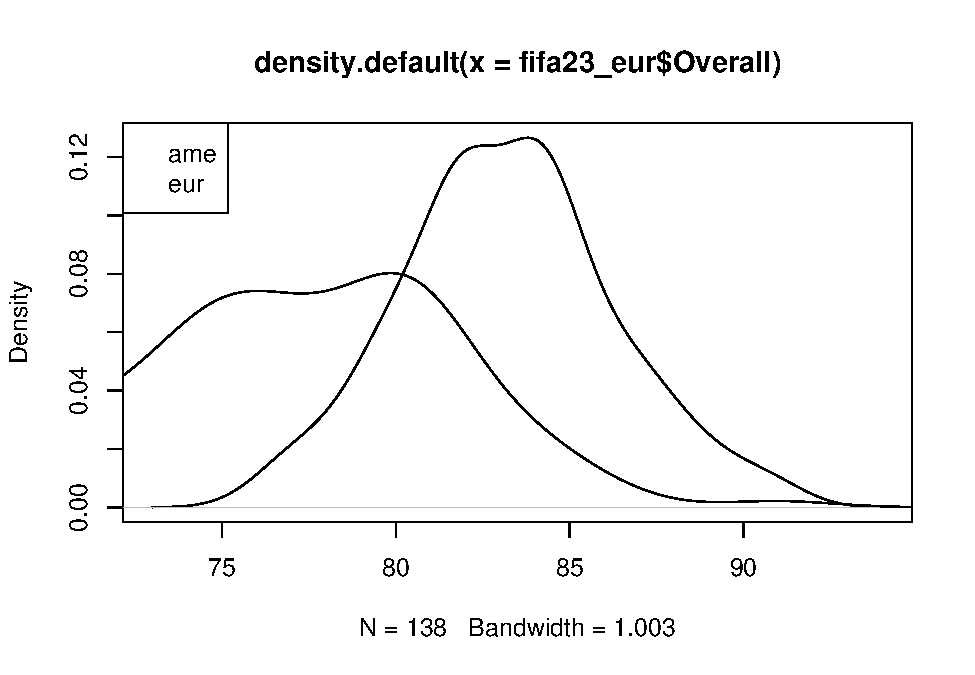
\includegraphics{taller_evaluable1_ENUNCIADO_22_23_files/figure-latex/unnamed-chunk-9-1.pdf}

\end{document}
